\chapter{La Réionisation}

Chronologiquement parlant, l'époque de Réionisation\index{Réionisation} désigne la dernière grande transition cosmologique vécue par l'Univers. Ce terme de Réionisation désigne la période durant laquelle le gaz d'hydrogène\index{hydrogène} du milieu intergalactique\index{IGM}\sidenote{on distingue aussi la Réionisation de l'hélium, plus tardive et que l'on ne mentionnera pas dans ce chapitre} retourne pour l'essentiel à l'état ionisé alors qu'il avait pourtant recombiné lors de l'émission du fond diffus cosmologique. Cette période prend place environ 1 milliard d'années après le Big-Bang \sidenote{pour un redshift $z\sim 6$}, et est le produit de l'apparition des première sources de lumières astrophysiques. Avec la naissance de ces premières sources au sein des précurseurs des galaxies actuelles, la Réionisation marque ainsi le début de l'astrophysique non-linéaire, complexe.

\section{Chronologie de la Réionisation et propriétés globales}
Environ 380 000 ans après le Big-Bang, la Recombinaison\index{Recombinaison} laisse place à un Univers rempli d'hydrogène neutre qui va refroidir sous l'effet de l'expansion. Cette période est désignée sous le terme 'd'âges sombres'\index{age@âges sombres} car l'Univers est rempli de gaz n'ayant pas encore réussi à former les premières sources de rayonnement. Ces dernières apparaissent quelques centaines de millions d'années après le Big-Bang\sidenote{probablement vers des redshifts $z\sim30$} : on compte parmi ces sources les premières étoiles\index{etoiles@étoiles} et les premiers noyaux actifs de galaxies\index{noyau actif de galaxie}, dont le moteur central est un trou noir\index{trou noir} supermassif en accrétion.

\begin{figure}[htbp]
	\centering
		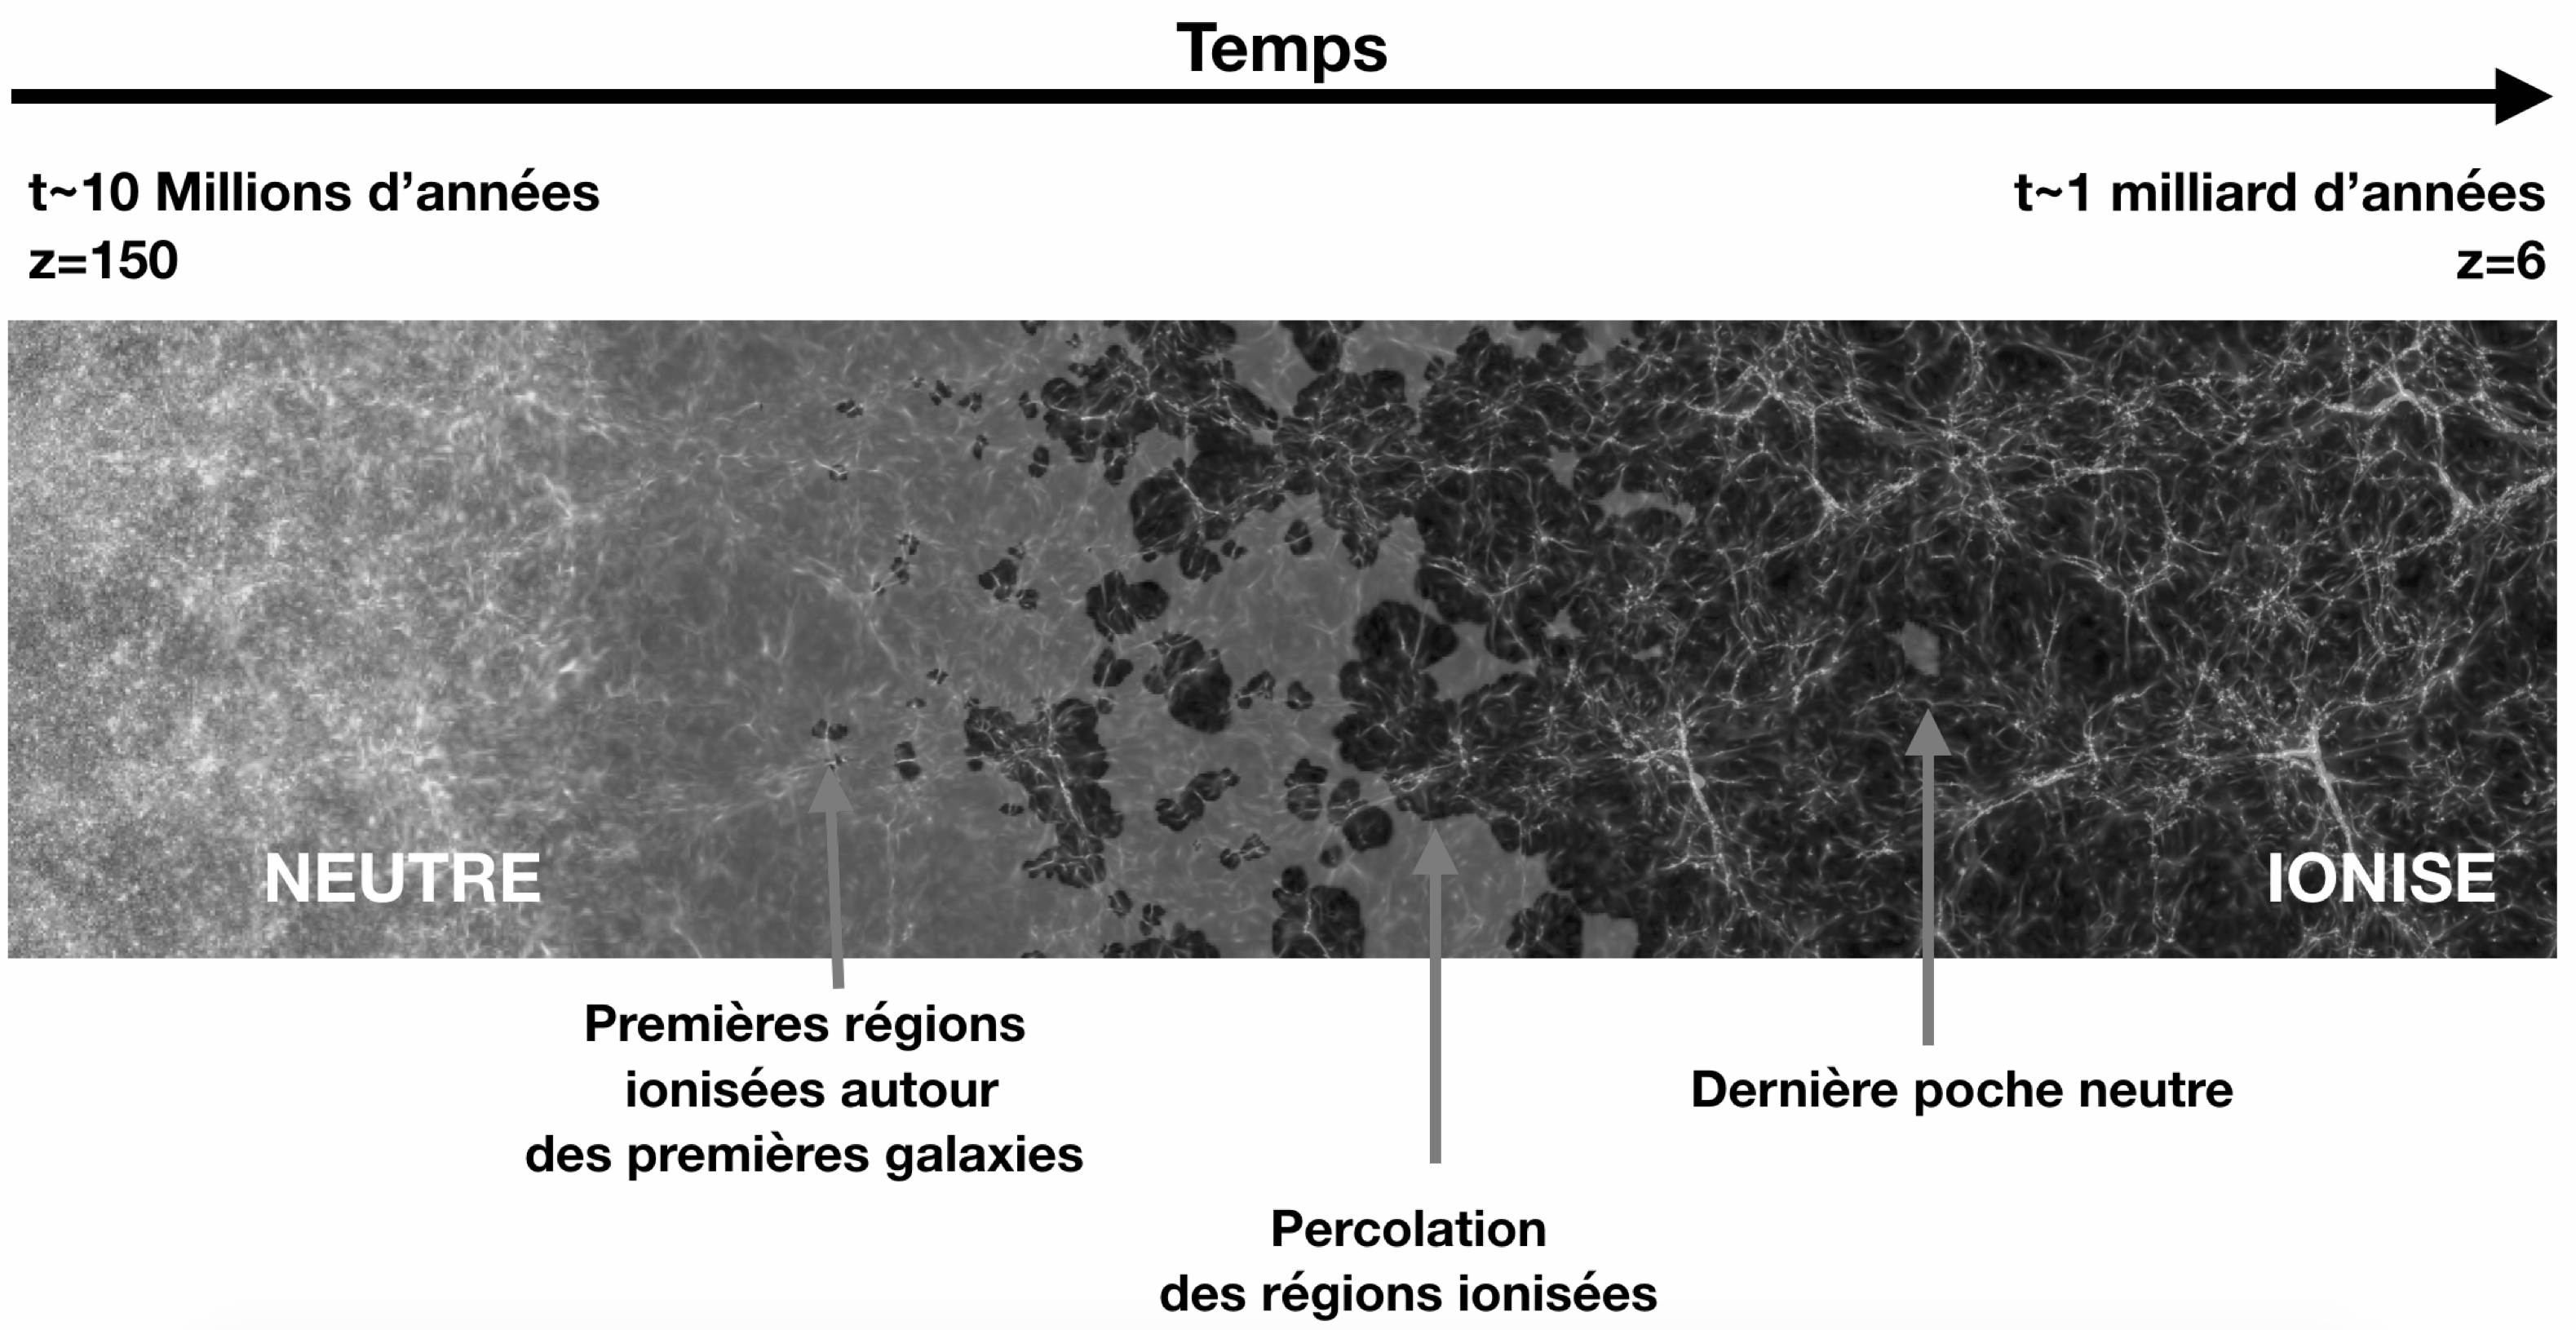
\includegraphics[height=10cm]{figs/frisereion.png}
		\caption[Chronologie de la Réionisation]{La chronologie de l'époque de Réionisation. Les régions neutres sont claires et les régions ionisées sont sombres.}
	\label{f:frisereion}
\end{figure}

Ces sources de rayonnement vont produire entre autre du rayonnement ultra-violet\index{fond UV}, capable d'ioniser l'hydrogène cosmique, dont l'énergie de liaison vaut 13.6 eV. Chaque source va alors se voir entourée d'une région ionisée\index{ionisation}, une 'bulle' appelée région HII\index{région HII}. Sous l'apport continu de photons ionisants par les sources, ces bulles vont grandir et compte tenu de l'apparition de plus en plus de sources, ces bulles vont devenir de plus en plus nombreuses. In fine, un réseau de région HII va s'établir puis percoler pour conduire à un Univers totalement ionisé, environ 1 milliard d'années après le Big-Bang. Après cette transition, la fraction résiduelle d'atomes neutres est de l'ordre de $0.01\%$\index{IGM!fraction ionisée}.

En parallèle, cette ionisation va s'accompagner d'un réchauffement du gaz : chaque ionisation va également transmettre de l'énergie à la matière. La température typique du gaz diffus en fin de Réionisation est de l'ordre de 10 000 K \index{IGM!température}~: cette température correspond au seuil de refroidissement de l'atome d'hydrogène\sidenote{voir le chapitre dédié à la formation des petites structures}. Plus chaud, le gaz va évacuer de l'énergie via des processus atomiques, plus froid le gaz est libre de voir sa température augmenter.

\section{Les régions HII}

\begin{figure}[htbp]
	\centering
		\includegraphics[height=10cm]{figs/dX.png}
		\caption[Le réseau de bulles ionisées de la Réionisation]{La distribution de gaz ionisé dans un Univers en cours de Réionisation d'après un calcul de simulation numérique. Les régions claires sont ionisées et chaudes, centrées autour des régions qui forment des étoiles. L'image fait environ 90 Mpc de côté et représente un Univers à z=8 environ à mi-Réionisation.}
	\label{f:dX}
\end{figure} 

La création de 'bulles' ionisées autour des premières sources est le processus élémentaire à l'origine de la Réionisation complète de l'Univers : ces bulles sont appelées régions HII\index{région HII}\sidenote[][-2cm]{HI étant une dénomination de l'hydrogène neutre. Par analogie on parle de HeI, HeII et HeIII pour désigner l'hélium neutre, ionisé une fois et deux fois.}. L'étendue de ces régions est régie par la compétition entre 2 effets aux conséquences opposées:
\begin{itemize}
\item d'une part la production de photons ionisants par une source\index{ionisation}. Ces photons  grignotent le gaz neutre et tendent à faire grandir la région HII
\item d'autre part la tendance naturelle des électrons libres à recombiner\index{recombinaison} avec les noyaux pour reconstituer des atomes. Cette recombinaison a tendance à réduire la taille de ces régions ionisées.
\end{itemize}
Une simple équation permet de faire la synthèse de cette compétition \sidenote{$N_H$ désigne la densité numérique d'atomes d'hydrogène neutres (en m$^{-3}$), $N_{H+}$ celle d'atomes ionisés, $N_e$ celle des électrons libres}:
\begin{equation}
\frac{d n_H}{dt}=\alpha n_{H+}n_e -\Gamma n_H.
\end{equation}
Ici $\alpha(T)$ est le taux de recombinaison\index{taux de recombinaison} de l'hydrogène : il dépend de la température\sidenote{un gaz froid a tendance à recombiner plus efficacement} et possède les dimensions d'un volume par unité de temps. Cette quantité, et donc le terme associé dans cette équation différentielle, encode la capacité du gaz ionisé à redevenir spontanément neutre.  A l'inverse $\Gamma$ est le taux de photoionisation\index{taux de photoionisation} et dépend du nombre de photons ionisants produits et présents dans la bulle ionisée.

Plutôt que de raisonner en abondance de protons et d'électrons, il est d'usage d'introduire la fraction d'ionisation\index{fraction d'ionisation} $x$:
\begin{equation}
x=\frac{n_{H+}}{n_{H+}+n_H}
\end{equation}
qui renvoie simplement le fraction d'atomes ionisés par rapport au nombre total de noyaux d'hydrogène disponibles (sous forme atomique ou non). Cette fraction ionisée sera une quantité centrale pour décrire la Réionisation cosmologique. En négligeant la contribution des éléments autres que l'hydrogène au gaz cosmique\sidenote{on rappelle que son abondance est proche de $95\%$ en nombre} et en utilisant le principe d'équilibre des charges électrique, le terme de recombinaison peut s'écrire:
\begin{equation}
n_\mathrm{rec}=\alpha x^2 n^2
\end{equation}
où $n=n_{H+}+n_H$ désigne la densité totale de protons. Si la région est complètement ionisée, $x=1$ et ce terme devient simplement:
\begin{equation}
n_\mathrm{rec}=\alpha n^2.
\end{equation}
Si on modélise la région HII par une sphère de rayon $R$, le nombre total de recombinaisons par seconde à l'intérieur est donné par:
\begin{equation}
N_\mathrm{rec}=\frac{4}{3}\pi R^3\alpha n^2.
\end{equation}
Si ce nombre de recombinaisons est égal au nombre de photons ionisant produits par seconde $ \dot N_\mathrm{ion}$, la région ionisée ne peut s'agrandir et on obtient une sphère, stationnaire, dite de \textit{Strömgren}\index{sphère de Strömgren}\sidenote{du nom du scientifique ayant décrit pour la première fois ce processus}, dont le rayon $R_s$ satisfait:
\begin{equation}
\frac{4}{3}\pi R_s^3\alpha n^2=\dot N_\mathrm{ion}.
\end{equation}
Cette région HII, stationnaire, possède donc un rayon donné par :
\begin{equation}
R_s=\left(\frac{3 \dot N_\mathrm{ion}}{4\pi \alpha n^2}\right)^{1/3}.
\end{equation}
Plus la production de photons\index{photons} est importante, plus ce rayon est important et à l'inverse un milieu dense en atomes, ou recombinant plus facilement à cause d'une basse température, présentera un rayon stationnaire plus petit.

Le cas non-stationnaire, avec un front en cours de progression, est plus délicate à traiter. Une approche possible consiste à considérer qu'un observateur lié au front d'ionisation voit d'un côté de ce front un flux de masse neutre et de l'autre un flux de masse ionisée, contraint par le flux de photons ionisants local. Ces 2 flux doivent être égaux \sidenote{$m$ désigne la masse d'un atome d'hydrogène, $v$ la vitesse du front\index{vitesse!front d'ionisation} et $F_\mathrm{ion}$ le flux de photons ionisants}:
\begin{equation}
m n v = m F_\mathrm{ion}.
\end{equation}
La vitesse du front satisfait donc:
\begin{equation}
v=\frac{1}{n}\frac{\dot N_\mathrm{ion}(r_f)}{4\pi r_f^2}.
\end{equation}
Le taux de photoionisation disponible au niveau du front est le taux de photoionisation total moins le nombre de recombinaison à l'intérieur du front:
\begin{equation}
\dot N_\mathrm{ion}(r_f)=\dot N_\mathrm{ion}(0)-\frac{4}{3}\pi r_f^3\alpha n^2=\frac{4}{3}\pi \alpha n^2 (R_s^3-r_f^3),
\end{equation}
d'où l'équation différentielle sur la position du front $r_f$ :
\begin{equation}
3r_f^2\frac{d r_f}{dt}=\frac{dr_f^3}{dt}=\alpha n  (R_s^3-r_f^3).
\end{equation}

\begin{figure}[htbp]
	\centering
		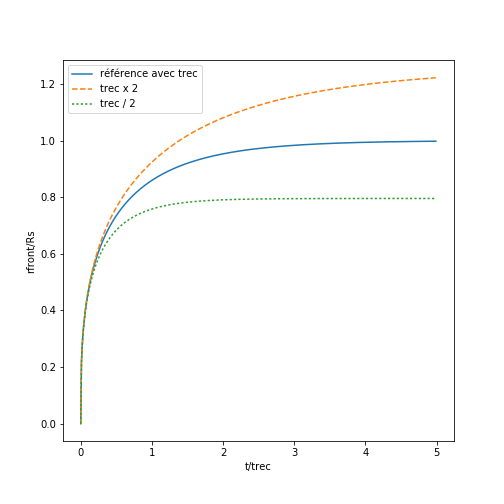
\includegraphics[height=10cm]{figs/strom.png}
		\caption[Évolution temporelle de la position d'un front ionisant]{Évolution temporelle du rayon d'une région HII. Les rayons sont exprimés en unités du rayon de Strömgren du modèle de référence, correspondant à l'état final stationnaire, tandis que les temps sont exprimés en temps de recombinaison. On constate que les modèles à temps de recombinaison courts, donc efficaces, ont des rayon d'équilibre plus petits et les fronts sont stoppés plus rapidement.}
	\label{f:strom}
\end{figure}

La solution sur la position du front \sidenote[][-2cm]{en posant $y=(r_f/R_s)^3$, on peut reconnaître une simple équation différentielle du premier ordre avec second membre constant} est alors donnée par:
\begin{equation}
r_f(t)=R_s(1-e^{-t/t_\mathrm{rec}})^{1/3},
\end{equation}
la position du front converge vers le rayon de la sphère de Strömgren\index{sphère de Strömgren}, sur une durée caractéristique $t_\mathrm{rec}=(\alpha n)^{-1}$, qui n'est autre que le temps de recombinaison\index{temps!recombinaison} caractéristique du gaz. Si le gaz recombine, le front ionisant stoppe rapidement et le rayon se stabilise. A l'inverse un gaz diffus ou chaud, à faible pouvoir de recombinaison va voir ses fronts se propager aisément. Dans la figure \ref{f:strom}, on constate dans tous les cas que la progression initiale des fronts est toujours rapide puis tend à ralentir lorsque les recombinaisons commencent à faire effet (pour $t\sim t_\mathrm{rec}$). La température typique du gaz intergalactique \index{IGM!température}est de l'ordre de $T=10 000 K$, tandis que les densités physiques d'atomes pour des filaments de gaz intergalactiques sont environ de 1000 atomes/$m^3$. Dans ces conditions, les temps de recombinaison typiques sont de l'ordre de la centaine de millions d'années.

\section{Éléments de transfert radiatif}

Bien sûr le cas de la région HII décrit précédemment est idéalisé : dans le cas cosmologique la densité d'atomes n'est pas homogène, le gaz réagit dynamiquement à la présence du front, la température n'est pas constante et bien sûr l'expansion de l'Univers conduit à une densité qui n'est pas constante au cours du temps. Par ailleurs, les sources de rayonnement ne sont pas stationnaires, elles vivent des histoires compliquées et s'influencent les unes les autres. Pour résoudre le problème dans toute sa complexité, il faut utiliser des simulations cosmologiques capables de modéliser la physique du \textit{transfert} radiatif\index{transfert radiatif}, la physique de l'interaction de la matière avec le rayonnement. 

La base du transfert du rayonnement est la résolution de l'équation du transfert radiatif qui décrit l'évolution de l'intensité du rayonnement $I_\nu({\bf x},{\bf n} ,t)$ \sidenote{$I_\nu$ désigne l'intensité spécifique du rayonnement, $S_\nu$ les sources de rayonnement et $\kappa_\nu$ l'absorption}:
\begin{equation}
\frac{1}{c}\frac{\partial I_\nu}{\partial t}+{\bf n} \frac{\partial I_\nu}{\partial {\bf x}}=S_\nu - \kappa_\nu(\bf x) I_\nu.
\end{equation}
En plus du temps, cette intensité dépend de la position $x$, de la fréquence $\nu$ et de la direction de propagation $\bf n$~: on se trouve donc face à un problème de très grande dimensionnalité (7 dimensions)~: l'équation du transfert est pour l'essentiel une équation de conservation de la fonction de distribution des photons\index{photons!distribution} dans l'espace des phases. Fondamentalement, cette équation est une variation de l'équation de Boltzmann.

Il existe plusieurs manières de 'simplifier' sa résolution, en réduisant sa dimensionnalité. L'une des plus communes consiste à considérer une source à l'origine seulement\sidenote{on néglige ainsi les sources diffuses, comme celles dues à la recombinaison atomique} et à supposer que la lumière est instantanément\sidenote{$c\rightarrow \infty$} et partiellement absorbée en chaque point de son trajet depuis l'origine. Le long de la direction de propagation, l'équation du transfert se réduit alors à:
\begin{equation}
 \frac{\partial I_\nu}{\partial {\bf x}}=- \kappa_\nu(\bf x) I_\nu,
\end{equation}
où $\kappa_\nu(\bf x)^{-1}$ apparaît comme une mesure de la distance sur laquelle l'absorption a lieu, tel un libre parcours-moyen\index{libre parcours moyen}.

Le long du rayon, la solution est alors:
\begin{equation}
I_\nu(x)=I_\nu(x=0)e^{-\int_0^x \kappa_\nu dx}=I_\nu(x=0)e^{-\tau},
\end{equation}
cette solution est une classique exponentielle décroissante, dont la grandeur caractéristique est \textit{l'opacité} $\tau$ mesurée le long du rayon\index{opacité}. Plus cette opacité est importante le long de la direction de propagation, plus le rayonnement est atténué. Si on dispose d'un modèle de distribution des sources dans l'espace, on peut donc tracer des rayons\index{transfert radiatif!lancer de rayons} dans toutes les directions et calculer cette opacité le long de tous ces rayons : cette donnée permet d'évaluer la quantité de rayonnement partout et donc la distribution spatiale du taux de photoionisation partout pour modéliser la Réionisation.

Une autre approche consiste à prendre les moments\index{transfert radiatif!moments}\sidenote{notons qu'en hydrodynamique la densité et le flux de masse (donc la densité d'impulsion) sont les moments de la fonction de distribution $\rho =\int dv f$ et $\rho v= \int dv v f$} de l'équation du transfert radiatif, pour évaluer la densité ou le flux de rayonnement\index{flux!rayonnement} par exemple:
\begin{eqnarray}
N_\nu&\sim&\int I_\nu d^3{\bf n}\\
{\bf F}_\nu&\sim&\int {\bf n} I_\nu d^3{\bf n}
\end{eqnarray}
Ces quantités ne dépendent plus que de la position et satisfont leurs propres équations de conservation\sidenote[][-1cm]{en négligeant les termes sources}:
\begin{eqnarray}
\frac{1}{c}\frac{\partial N_\nu}{\partial t}+\frac{\partial {{\bf F}_\nu}}{\partial {\bf x}}&=&-\kappa N_\nu\\
\frac{1}{c}\frac{\partial {\bf F}_\nu}{\partial t}+\frac{\partial {{\bf P}_\nu}}{\partial {\bf x}}&=&-\kappa' {\bf F}_\nu.
\end{eqnarray}
On a donc affaire à un système d'équations dites hyperboliques, similaires aux équations de l'hydrodynamique\sidenote{conservation de la masse et équation d'Euler} et qu'on peut alors résoudre à l'aide des même techniques. Toutefois, cela nécessite de fermer le système d'équation avec une équation d'état du rayonnement liant la pression\index{pression!rayonnement} radiative $\bf P$ avec la densité de rayonnement par exemple~: il existe toute une série de modèles qui fournissent ce type de relation en fonction du problème physique considéré. Plus radicalement, on peut aussi se contenter de l'équation de conservation de la densité de rayonnement et imposer que le flux radiatif soit simplement lié au gradient de cette densité:
\begin{equation}
{\bf F_\nu}=-c\nabla N_\nu,
\end{equation}
pour obtenir une \textit{équation de diffusion} dans laquelle le rayonnement va alors 'couler' des régions brillantes aux régions éteintes:
\begin{equation}
\frac{\partial N_\nu}{\partial t}+c^2\frac{\partial^2 {N_\nu}}{\partial {\bf x}^2}=-\kappa N_\nu.
\end{equation}
 Simple à mettre en place, ce modèle souffre toutefois de l'impossibilité de créer des ombres derrières des absorbants denses.

\section{Observer la Réionisation de l'Univers}
L'époque de Réionisation\index{Réionisation} s'achève à $z\sim 6$, correspondant à un Univers âgé environ de 1 milliard d'années. Son début est beaucoup plus incertain : la transition démarre avec l'apparition des premières sources, très probablement des étoiles, mais l'instant de leur apparition n'est pas connu avec certitude. On pense aujourd'hui qu'il faut quelques centaines de millions d'années pour que le gaz puisse acquérir les conditions lui permettant de former ces premières sources, correspondant à des redshift $z\sim 30- 50$. Ces époques sont particulièrement reculées, donc distantes, et sont donc difficiles à observer.  On dispose aujourd'hui de 2 grandes observations qui démontrent que la transition a bien eu lieu : la forêt Lyman-$\alpha$ et l'étude du fond diffus cosmologique.

\subsection{Le milieu intergalactique, la Forêt Lyman-Alpha}
La première observation 'canonique' de la Réionisation est l'étude de la forêt Lyman-Alpha\index{forêt Lyman-$\alpha$}. Ce terme désigne les spectres de sources brillantes lointaines (généralement des quasars) qui présentent des systèmes de raies d'absorption denses aux fréquences plus élevées que la raie Lyman-Alpha de l'hydrogène\index{hydrogène}\sidenote{dont la longueur d'onde est 121.6 nm}. Le principe qui conduit à l'apparition de ces raies est simple : ces sources possèdent un spectre continu et une raie Lyman-alpha en émission. Au cours de leur propagation les photons associés vont se décaler vers le rouge à cause de l'expansion cosmique. Après la Réionisation, l'hydrogène cosmique est en très grande majorité ionisé et ne peut en général absorber ces photons. Si toutefois l'un d'entre eux rencontre un nuage d'hydrogène \textit{neutre} au sein du milieu intergalactique, ce dernier va générer une raie\index{raie d'absorption} en absorption à 121.6 nm dans son référentiel. Toutefois, comme le spectre de la source lointaine perçu par le nuage est décalé vers le rouge, l'absorption va se faire à une fréquence plus élevée que celle de la raie en émission. Si jamais un second nuage se trouve sur la ligne de visée, une autre absorption va s'ajouter ~: comme le spectre de la source lointaine s'est encore d'avantage rougi\index{rougissement}, cette raie d'absorption supplémentaire se placera dans les parties plus bleues, à plus haute fréquence que la raie créée par le premier nuage et que celle de la raie en émission. Par extension si de multiples nuages sont présents sur la ligne de visée, chacun d'entre eux va générer une raie en absorption qui prises globalement donne l'apparence d'une 'forêt' de raies.

\begin{figure}[htbp]
	\centering
		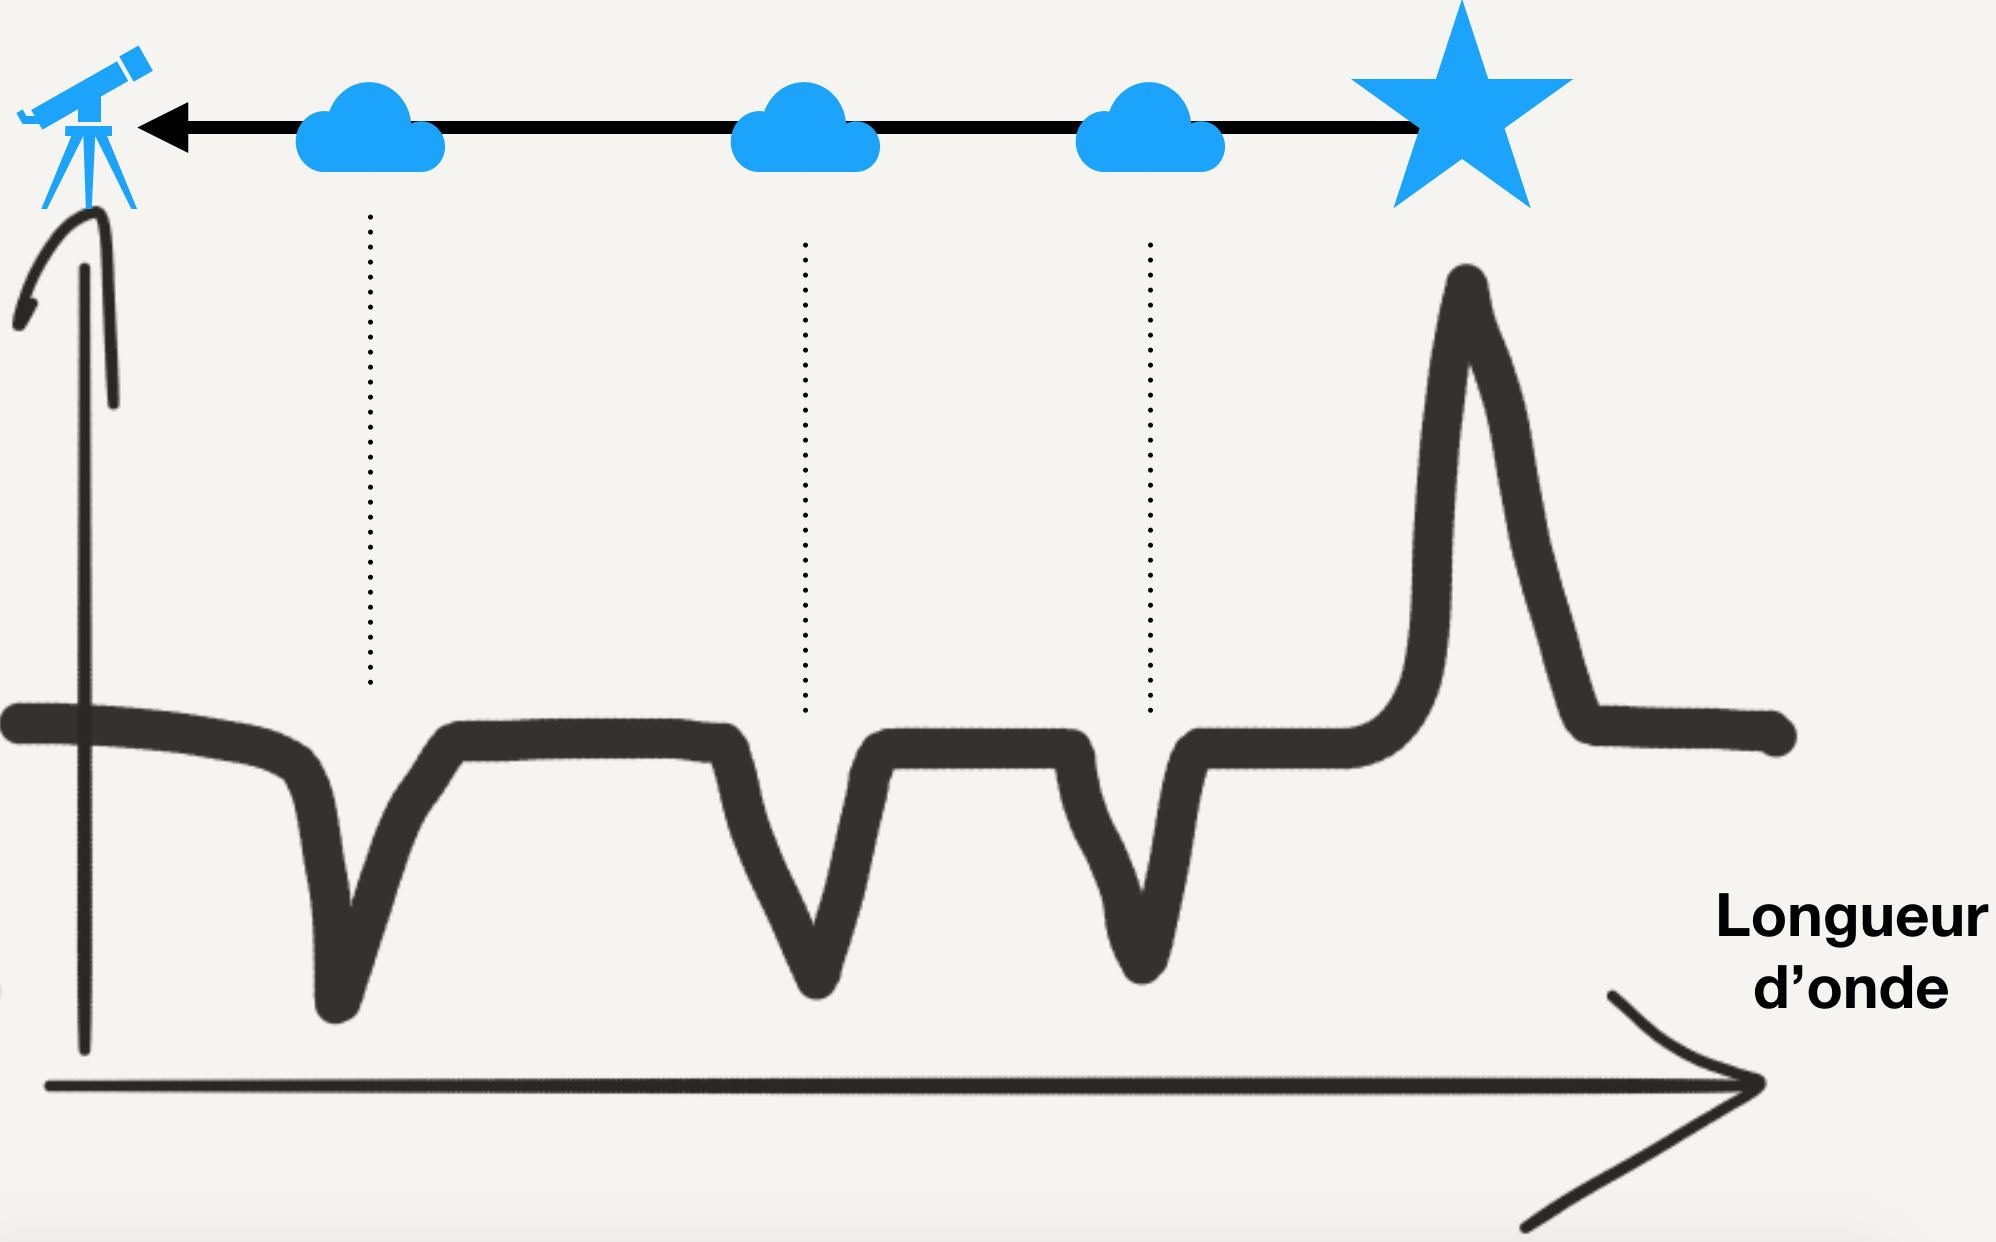
\includegraphics[height=12cm]{figs/lya.png}
		\caption[Principe de la forêt Lyman-$\alpha$]{La forêt Lyman-$\alpha$ est un ensemble de raies d'absorption créées par des nuages neutres absorbants le long de la ligne de visée vers une source lointaine brillante. Chaque nuage perçoit le spectre de la source de façon décalée à cause de l'expansion cosmologique et va donc placer une raie d'absorption à sa propre fréquence correspondant à 121.6 nm dans son référentiel.}
	\label{f:lya}
\end{figure}

La forêt Lyman-Alpha est un outil particulièrement puissant puisqu'elle permet de tracer la distribution spatiale et les propriétés (température par exemple) des nuages neutres de gaz le long de la ligne de visée. On a donc accès à l'état du milieu intergalactique\index{IGM} sur toute une gamme d'époques. Si par ailleurs on dispose de multiples lignes de visées, il est possible de réaliser de la \textit{tomographie}\index{tomographie}, c'est à dire une reconstruction 3D de la structure du milieu intergalactique, entre ces sources et nous.

Que se passe-t-il si la source émet ses photons dans une époque antérieure à la Réionisation ? Au lieu d'avoir une discontinuité de nuages neutres absorbants, \textit{l'ensemble} du milieu intergalactique\index{IGM} , qui est neutre, est capable de produire une absorption. L'observateur constate alors une continuité d'absorptions aux longueurs d'ondes plus courtes que l'émission Lyman-$\alpha$ et dans les cas les plus extrêmes, la transmission est proche de zéro : le spectre présente alors un \textit{Gunn-Peterson Through}\index{Gunn-Peterson}\sidenote{on pourra le traduire par 'Tunnel' Gunn-Peterson}, caractérisé par une absence de signal sur une grande gamme de longueurs d'ondes. C'est précisément ce qui est obtenu lorsque l'on observe des spectres de quasars\index{quasar} de plus en plus lointains, de plus en plus enfouis dans l'époque de Réionisation~: la disparition graduelle de la forêt indique la mise en place d'un Univers rempli de gaz neutre absorbant aux alentours d'un redshift $z\sim 6$.
\begin{figure}[htbp]
	\centering
		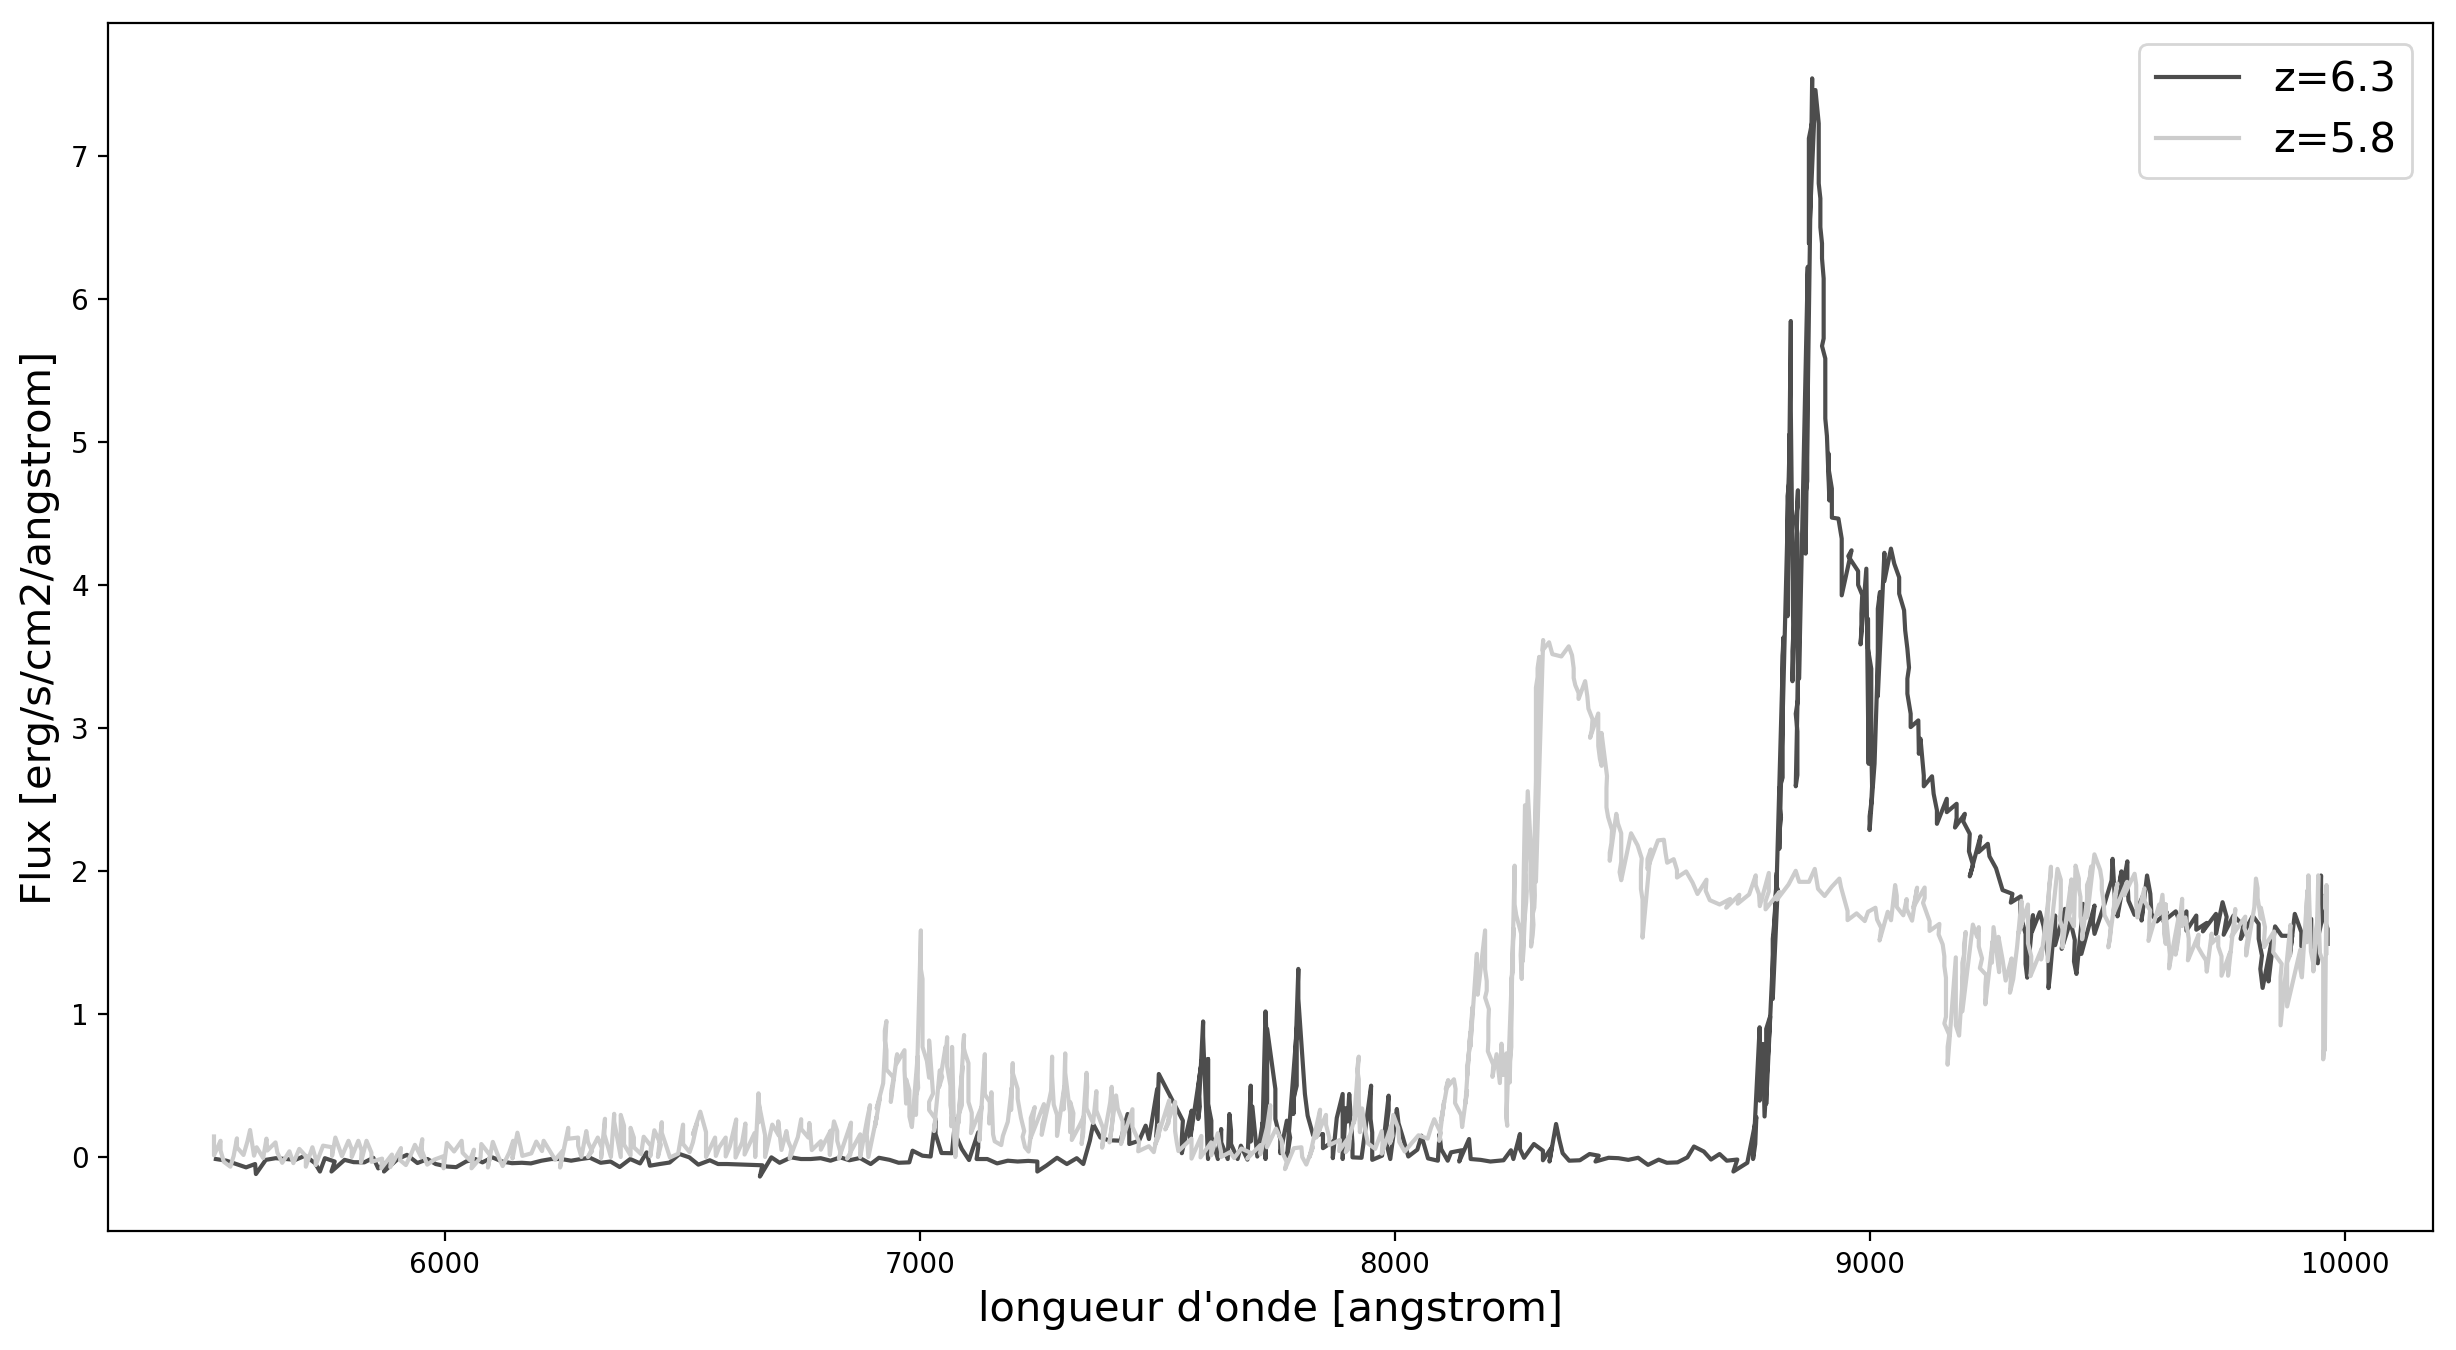
\includegraphics[height=12cm]{figs/Becker01.png}
		\caption[Spectres de quasars durant la Réionisation]{Un échantillon de spectres de quasars émettant durant l'époque de Réionisation. Le quasar à grand redshift émet son rayonnement avant que la Réionisation ne soit terminée : aux fréquences plus élevées que la raie en émission, on note un signal très faible voire inexistant, c'est une manifestation du \textit{Gunn-Peterson Through} dû à la présence de gaz neutre en quantité importante. Par contraste, le quasar à plus bas redshift émet après la période de Réionisation dans un Univers déjà ionisé : la transmission est plus importante, le signal de la forêt Lyman-Alpha est plus marqué sans jamais descendre à des niveaux aussi bas que pour le premier spectre.}
	\label{f:fan06}
\end{figure}

\subsection{L'opacité Thomson du CMB}
La Réionisation\index{Réionisation!fond diffus}\index{fond diffus} va produire des électrons libres aux alentours d'un redshift de 6, un milliard d'années après le Big-Bang. Or ces électrons vont naturellement avoir tendance à interagir avec les photons du fond diffus cosmologique\index{fond diffus cosmologique} tandis que ces derniers volent vers un observateur terrestre \sidenote[][4cm]{de façon analogue à l'effet Sunyaev-Zeldovich où ce sont les électrons libres des amas de galaxies à bas redshift qui font office de cibles}: ce processus de diffusion dit Thomson\index{diffusion Thomson} va affecter la structure angulaire du fond diffus cosmologique, particulièrement aux grandes échelles. Cet effet peut-être évalué quantitativement et donc mettre des contraintes sur l'histoire de la Réionisation.

\begin{figure}[htbp]
	\centering
		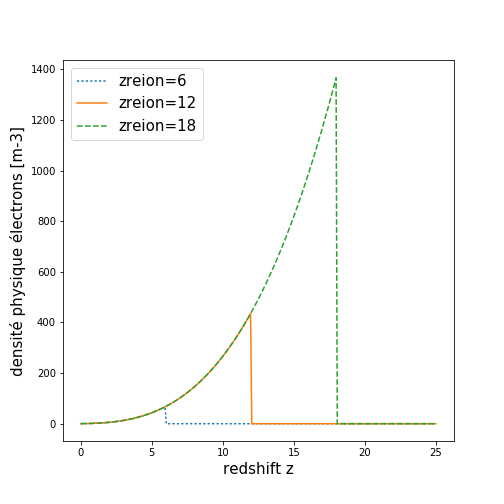
\includegraphics[height=10cm]{figs/ne.png}
		\caption[La densité cosmique d'électrons ]{La densité physique d'électrons pour 3 modèles simples de Réionisation instantanée et complète. L'opacité Thomson, le taux d'interaction des électrons avec les photons du CMB, est donnée par l'intégrale de cette courbe : plus la Réionisation est précoce, plus l'opacité est importante.}
	\label{f:nereion}
\end{figure}

La quantité importante s'appelle l'opacité Thomson\index{opacité!fond diffus} et est calculée de la manière suivante:
\begin{equation}
\tau_\mathrm{th}=\int_{z_\mathrm{rec}}^{z=0} c \sigma_T n_e(z) dt
\end{equation}
et revient de fait à calculer une histoire intégrée de la production d'électrons libre $n_e$ au cours de l'histoire cosmique. En théorie, le calcul de la valeur de l'opacité dépend de l'histoire détaillée de Réionisation mais il est facile de comprendre le comportement qualitatif de cette quantité à partir d'un modèle simple. En effet, supposons que la Réionisation soit parfaite de telle manière à ce que tous les atomes d'hydrogène soient ionisés et qu'elle soit instantanée. Dans ce cas la densité comobile d'électrons libres est simplement constante et vaut \sidenote{on considère que l'hélium est négligeable}:
\begin{equation}
n_\mathrm{e,com}=\frac{\Omega_b \rho_c}{m_p}.
\end{equation}
La densité \textit{physique} d'électrons, celle nécessaire au calcul de $\tau_\mathrm{th}$, est donc simplement nulle avant la Réionisation et après la Réionisation vaut (voir Fig \ref{f:nereion}):
\begin{equation}
n_e(z<z_\mathrm{reion})=\frac{\Omega_b \rho_c}{m_p} \frac{1}{(1+z)^3}.
\end{equation}
La valeur de l'opacité vaut donc:
\begin{equation}
\tau_\mathrm{th}=\int_{z_\mathrm{rerion}}^{z=0} c \sigma_T\frac{\Omega_b \rho_c}{m_p} \frac{1}{(1+z)^3}  |\frac{dt}{dz}| dz.
\end{equation}

Plus le redshift de Réionisation est élevé (plus la transition est précoce) plus la valeur de $\tau_\mathrm{th}$ est importante. De fait les premières mesures de cette quantité par le satellite WMAP, donnait des valeurs de $\tau_\mathrm{th}\sim 0.17$ correspondant à des redshifts de Réionisation proches de $17$. Comparés à ceux obtenus par la technique des spectres de quasars, la tension était particulièrement forte entre ces 2 types de sondes de la Réionisation. Depuis, les mesures successives, via le satellite WMAP ou Planck\index{Planck!satellite} on ramené cette quantité à des valeurs plus raisonnables, de l'ordre de $\tau_\mathrm{th}\sim 0.068$ ce qui correspond à des redshifts de \textit{mi-Réionisation} de l'ordre de 8 : cette valeur est bien plus compatible avec celle mesurée via la forêt Lyman-$\alpha$. Toutefois, et de façon un peu paradoxale, une faible valeur de $\tau_\mathrm{th}$, donc une Réionisation plus tardive, a tendance à rendre le CMB moins pertinent pour l'étude de cette époque : en effet, une faible valeur indique un faible couplage entre les électrons de la Réionisation et les photons du CMB, et par extension ces photons sont moins sensibles à cette transition. Physiquement la raison en est simple~: une Réionisation tardive implique une densité physique d'électrons libres plus faibles que celle qui aurait été obtenue pour une transition précoce.

%\begin{figure}[htbp]
%	\centering
%		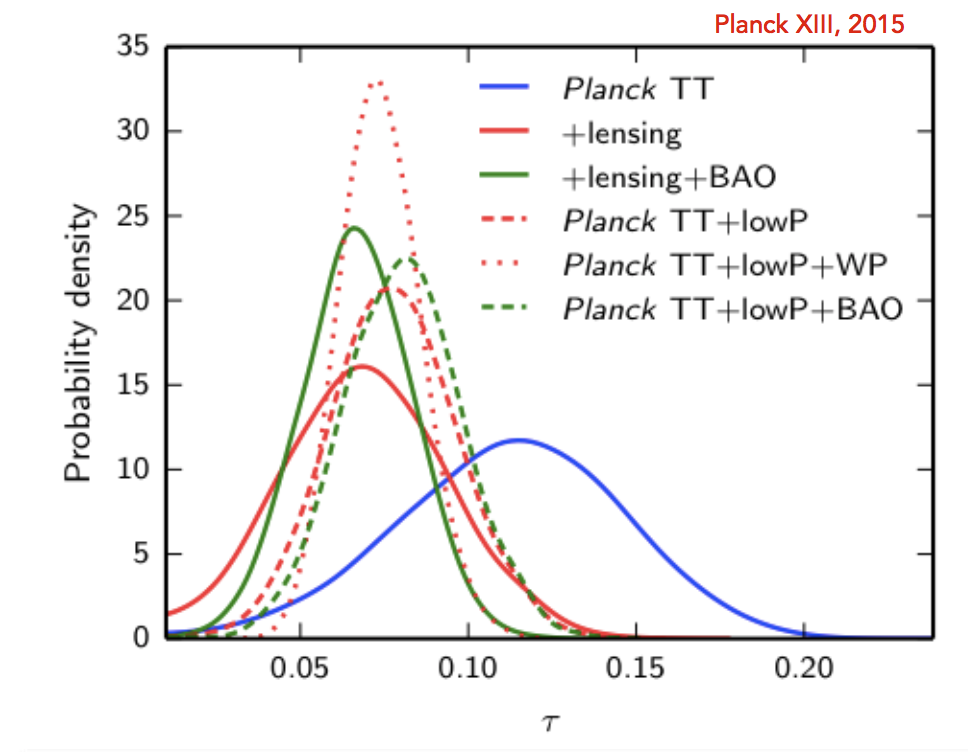
\includegraphics[height=12cm]{figs/tau.png}
%		\caption[L'opacité Thomson du CMB]{La distribution des valeurs possibles de $\tau_\mathrm{th}$ d'après les mesures du satellites Planck. Les différentes courbes représentent les différentes estimations en considérant soit les données Planck en température seules (courbes bleues) soit en les couplant à d'autres mesures (par exemple les BAOs dans la distribution des galaxies) pour contraindre davantage cette mesure. La meilleure estimation donne $\tau_\mathrm{th}\sim 0.066 \pm 0.016$ équivalant à un redshift de mi-Réionisation proche de 8.8. Figure extraite de Planck XIII.}
%	\label{f:tau}
%\end{figure}

\subsection{le signal à 21 cm}
 Contrairement aux 2 mesures précédentes, celle-ci n'a pas encore été réalisée dans le cas de la Réionisation mais elle est des plus prometteuses. Il s'agit de détecter le signal émis directement par le gaz d'hydrogène neutre, à la longueur d'onde de 21 cm\index{signal à 21 cm}. Ce signal radio correspond à la transition entre les 2 états de spin de l'électron sur le niveau fondamental\sidenote[][-2cm]{on parle de transition hyperfine\index{transition hyperfine}} : clairement l'écart d'énergie entre les 2 configurations doit être très faible, et le rayonnement produit est à très basse énergie. Le signal à 21 cm du gaz neutre peut s'exprimer sous la forme d'une température de brillance:
 \begin{equation}
 \delta T_b \sim x_\mathrm{HI} (1+\delta) (1-\frac{T_\mathrm{CMB}}{T_S})(1+\frac{1}{H}\frac{d v_r}{dr})^{-1}.
 \end{equation}
 Ce signal est extrêmement riche physiquement. Il dépend de l'état d'ionisation de l'hydrogène : un gaz complètement ionisé ($x_\mathrm{HI}=0$) donne un signal nul, comme attendu, et au cours de la Réionisation, la mise en place d'un réseau de bulles ionisées doit donc directement se manifester dans ce signal radio par sa disparition progressive. Il dépend aussi directement de la densité locale de gaz (via la surdensité $\delta$). Plus subtil, il dépend de la température de spin\index{température!spin}, c'est à dire du niveau d'occupation des niveaux hyperfins : cette température est une mesure de l'efficacité du pompage des états vers le niveau excité. Le mécanisme de pompage le plus pertinent dans ce contexte est l'absorption et la ré-émission de photons Lyman-$\alpha$ : ce mécanisme couple la température de spin avec celle du gaz mais requiert de tels photons et donc des étoiles.  En l'absence de photons Lyman-$\alpha$\index{photons!Lyman-$\alpha$}, les processus collisionnels au sein du gaz peuvent également produire du pompage, mais le régime de densité requis pour que cela soit efficace n'existe que pour des redshifts au-delà de ce qui est observable dans un futur proche ($z>40$) : dans cette situation on a à nouveau $T_S\sim T_\mathrm{gaz}$. Notons que le signal se mesure comparativement à la température du CMB $T_\mathrm{CMB}$\index{fond diffus!signal à 21 cm} ~: si la température de spin est égale à celle du fond diffus\sidenote{qui est de l'ordre de la dizaine de K aux redshifts considérés avec $T=2.73(1+z)$ K}, le signal à 21 cm est invisible. Si la température de spin est plus élevée que celle du CMB, alors le signal est vu en émission ($\delta T_b >0$). Il sera vu en absorption dans le cas contraire. Pour finir, il dépend de la vitesse du gaz le long de la ligne de visée, et permet donc potentiellement de remonter à cette dynamique.

\begin{figure}[htbp]
	\centering
		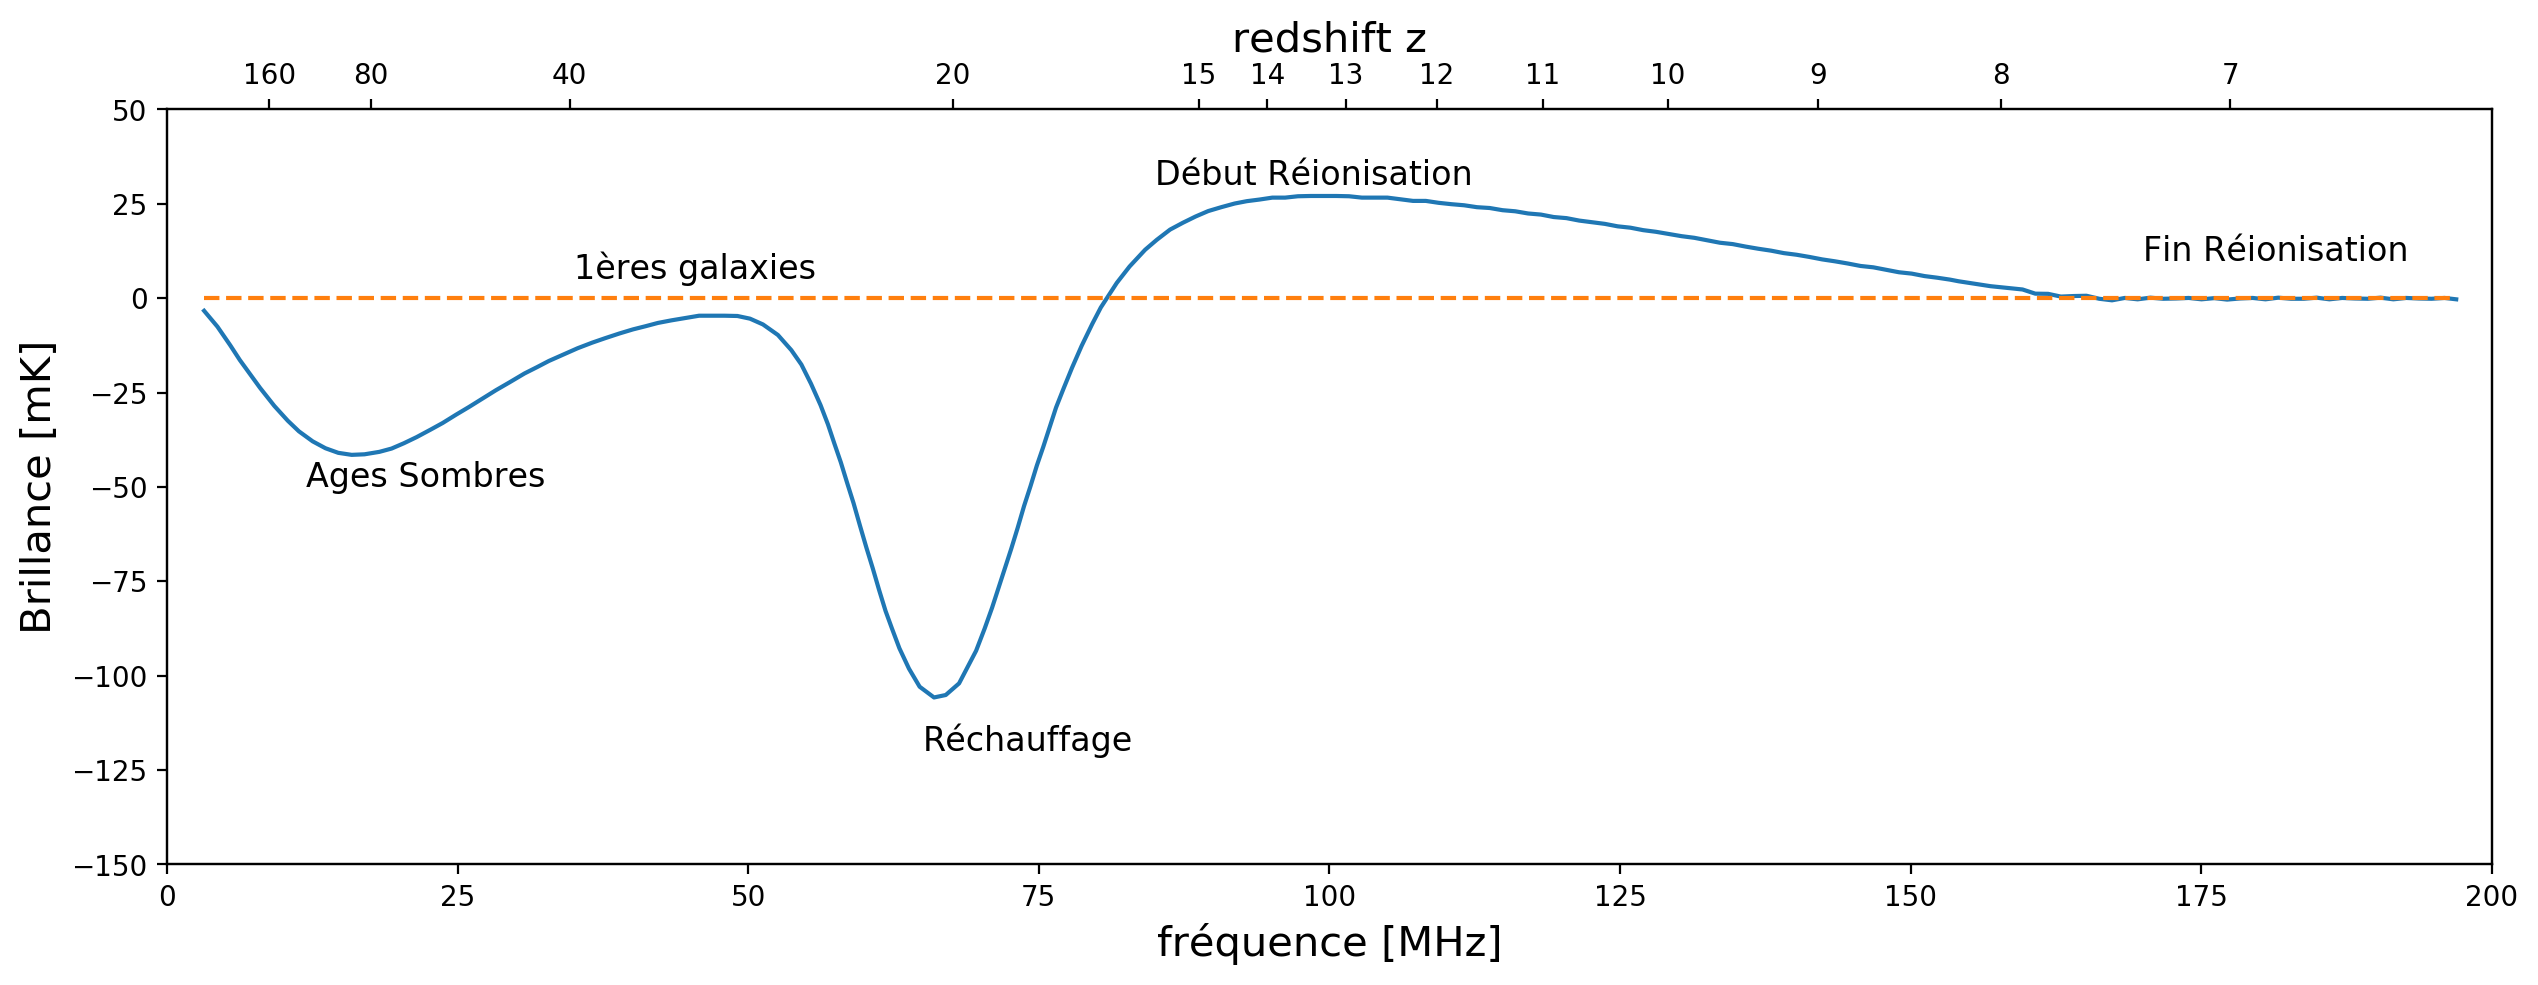
\includegraphics[height=12cm]{figs/21cm.png}
		\caption[L'histoire du signal à 21cm de la Réionisation]{Les différentes phases de l'émission à 21cm au cours de la Réionisation. Durant les âges sombres le signal est d'abord vu en absorption avant de commencer à disparaître. Il redevient visible lorsque les premières galaxies apparaissent. Dès que le chauffage du gaz par les premières sources de rayons X devient effectif, le signal va basculer dans une phase en émission. Puis il va redisparaître entre le début et la fin de la Réionisation. Figure inspirée de Pritchard \& Loeb 2012.}
	\label{f:21cm}
\end{figure} 

Cette richesse physique se traduit par une histoire compliquée pour le signal à 21 cm\index{signal à 21cm!Réionisation} moyen (cf Fig. \ref{f:21cm}). Dans un premier temps, durant les âges sombres\index{ages@âges sombres}, ce sont les collisions qui vont réaliser le couplage entre la température du gaz et celle de spin~: comme le gaz refroidit plus vite que le CMB \sidenote[][-2cm]{la température du gaz évolue en $(1+z)^{-2}$ tandis que celle du CMB évolue en $(1+z)^{-1}$}, le signal est vu en absorption. Tandis que la densité de gaz diminue, les collisions deviennent moins efficaces, la température de spin se découple de celle du gaz et se rapproche de celle du CMB, faisant disparaitre le signal. Il faut attendre que les premières sources, et en particulier les premières étoiles, se forment pour que leur production de rayonnement Lyman-$\alpha$ puisse à nouveau écarter la température de spin\sidenote{en la recouplant à celle du gaz} de celle du CMB, pour produire un signal en absorption. Par la suite, la production de rayons X, notamment par les premiers noyaux actifs de galaxies\index{noyau actif de galaxie}, va alors réchauffer le gaz jusqu'à le faire passer dans un régime en émission. A ce stade, les premières régions HII vont apparaitre et grignoter le gaz neutre émetteur, le signal va alors disparaitre jusqu'à ce que l'IGM\index{IGM} soit complètement réionisé.

La détection de ce signal et la réalisation de cartes de 21cm sur le ciel sont des objectifs majeurs du futur grand interféromètre radio SKA\index{SKA}\index{signal à 21 cm!SKA}. Prévu pour être installé sur 2 sites à partir de 2020, un en Australie et l'autre en Afrique du Sud, cet instrument sera capable d'imagerie, afin de voir la Réionisation en train de se faire, fournissant autant d'informations sur les sources de rayonnement, sur le milieu intergalactique, sur le processus de croissance des structures à ces époques, etc... On note qu'il suffit de changer de fréquence d'observation pour que l'instrument puisse accéder à un autre redshift et donc à une autre époque : non seulement SKA sera capable de cartographie, mais il sera en mesure d'extraire une évolution temporelle du processus. Pour finir, le même principe que la forêt Lyman-$\alpha$ peut être appliqué à la transition à 21cm, permettant de reconstruire la distribution de gaz le long de la ligne de visée d'une source radio intense~: on parle alors de forêt à 21cm\index{forêt à 21cm}, avec les même possibilités de tomographie que celles offertes par la forêt Lyman-$\alpha$. Cette technique nous est inaccessible pour l'instant, faute d'instruments suffisamment sensibles, mais SKA devrait pouvoir la rendre possible. 

\section{Réionisation et physique fondamentale}
L'époque de Réionisation est liée à la formation des premières sources et correspond à une époque reculée où se mettent en place les premiers processus d'astrophysique compliquée et non-linéaire. En corollaire, elle est donc proche des 'conditions initiales' et présente une physique qui n'a pas accumulé 13 milliards d'années d'évolution supplémentaire. La Réionisation est le lieu du démarrage de la formation des galaxies, et la compréhension de l'émergence de ces structures au tout début est un défi important : si on ne comprend pas les propriétés des galaxies à leur début quand les choses sont plus 'simples', difficile de prétendre à pouvoir le faire aux époques plus tardives, en particulier aujourd'hui, quand les choses ont eu le temps de devenir compliqué. En regardant comment la Réionisation du cosmos procède, sa géométrie et son évolution, on regarde une manifestation macroscopique, cosmologique, de la façon dont les premières galaxies sont créées aux 'petites' échelles et par extension on teste les modèles de formation des galaxies.

Comme expliqué dans la partie dédiée à la matière noire, le consensus actuel tourne autour d'une matière dynamiquement froide qui a comme conséquence une surproduction de petits halos en dessous de $10^9-10^{10} M_\odot$ par rapport aux observations. Une manière de répondre à ce défi est de considérer une matière noire 'tiède'\index{matière noire tiède}\sidenote{pouvant consister en un mélange de matière noire froide et chaude (neutrinos)} ou bien une matière noire en auto-interaction ou ayant un couplage avec le rayonnement électromagnétique faible mais non nul : toutes ces solutions diminuent la puissance aux petites échelles, réduisant la surproduction de petits halos et sont susceptibles d'imprimer une géométrie ou une évolution spécifique de la Réionisation. Le déroulé de la transition permettrait ainsi de sonder la nature de la matière noire.

Par ailleurs, la Réionisation affecte les galaxies, en remplissant l'Univers d'un rayonnement chauffant et ionisant\index{fond UV}. Comme vu précédemment, les petites galaxies de $10^9 M_\odot$ ont une température de viriel\index{température de viriel} de l'ordre de $10^4$ K, correspondant peu ou prou à la température à laquelle le gaz est amené par la propagation des fronts ionisants : ces petites galaxies vont se trouver dans l'impossibilité de conserver ce gaz à l'équilibre au sein de leur halo\sidenote{on parle de photo-évaporation} et ne pourront pas former d'étoiles. Cette suppression de la formation stellaire est une conséquence attendue de la Réionisation sur les petits objets : elle pourrait expliquer le désaccord majeur qui existe actuellement entre le nombre de galaxies satellites observé autour de galaxies comme la Voie Lactée et celui beaucoup plus grand prédit par les modèles de matière noire froide. Cette grande transition pourrait être un ingrédient essentiel du modèle $\Lambda CDM$ pour le rendre conforme aux observations faites aux échelles galactiques.

Enfin, l'expérience à 21cm américaine EDGES  a annoncé avoir détecté le premier signal radio de la Réionisation en 2018 : ce signal correspondrait à celui de la phase de couplage avec le rayonnement Lyman-$\alpha$ et au début du réchauffage, entre 70 et et 90 MHz c'est à dire des décalages vers le rouge $z$ compris entre 22 et 14. Si il est confirmé, ce signal est la première signature jamais détectée de l'apparition des premières étoiles, qui produisent le Lyman-$\alpha$. De façon inattendue, \textit{l'amplitude du signal} en absorption est bien plus importante que prévue, correspondant à une température du gaz cosmique quelques fois plus froid qu'anticipé, d'un facteur 2 ou 3\sidenote{typiquement une température de gaz de 3 K est mesurée alors qu'elle est attendue aux alentours 7-9 K}. Or la physique du gaz à cette époque est très simple et ce dernier ne refroidit que par expansion cosmologique : il faut donc invoquer un mécanisme exotique de refroidissement pour expliquer ces faibles températures. Peut-être s'agit-il de la marque d'une interaction avec la matière noire, qui pompe de l'énergie aux baryons ? Ce résultat et ces conclusions restent à confirmer à ce jour, mais ils montrent bien comment, dans une époque où les processus restent 'simples', un comportement légèrement non-orthodoxe peut conduire à des remises en causes importantes de notre compréhension physique.  
  
 